\chapter{Second-order effective charge model}
\addtocontents{toc}{\contentsline{chapter}{Second-order effective charge model}{\protect\pageref{annotation}}}
\label{ch:secondECM}

This chapter explains how to use the Green's function of the hydrogen equation to calculate second-order corrections to energies in the ECM. This includes corrections coming from adjusting the shapes of single-electron orbitals, as well as from electron-electron correlations. It also shows how to mitigate the divergences coming from the degeneracy of the hydrogen-like basis. Just like in the leading-order we avoid making any approximations beyond limiting the discussion to the second order of perturbation.

\section{Green's functions}
\label{sec:Green}

Second order correction to energy is given by the sum over all virtual multi-particle virtual states $\psi_k$
\begin{equation}
    \Delta E^{(2)} = \sum_k \frac{|\langle \psi^{(0)}|\widehat{W}|\psi_k\rangle|^2}{E^{(0)}-E_k}
\end{equation}
where the sum runs over all discrete and continuous states in the hydrogen-like basis  (see~\eqref{PertSeries}).

Since $W$ is a two-electron operator, only virtual states that differ by at most two single-electron orbitals contribute to the above sum. Hence for $|\psi^{0}\rangle = |\lambda_1...\lambda_n\rangle$, we have
\begin{equation} \label{SecondSigma}
    \Delta E^{(2)} = \sum_{k \neq l}^n \left(\sum_{\sigma} \frac{|\langle \lambda_k \lambda_l|\widehat{W}|\lambda_k \sigma \rangle|^2}{E_{\lambda_l}-E_\sigma} + \sum_{\sigma,\sigma'}\frac{|\langle \lambda_k \lambda_l|\widehat{W}|\sigma \sigma' \rangle|^2}{E_{\lambda_k}+E_{\lambda_l}-E_\sigma-E_{\sigma'}}\right)
\end{equation}
where $\sigma$ denotes the single-electron virtual states of the hydrogen-like basis.

We will refer to the first of these two terms as the single-electron second-order correction, denoted $\Delta E^{(2)}_{\rm{single}}$ and to the second as the double-electron second-order correction, denoted $\Delta E^{(2)}_{\rm{double}}$. Physically, the single-electron correction represents the adjustment of the shapes of single-electron orbitals, while the double-electron correction is related to the correlations between electrons.

At a first glance these corrections may seem complicated, but all of the above sums can be expressed in terms of the Green's function \footnote{This is a slight abuse of notation, as the sum includes all discrete and continuous spectra of the given basis. For example, in the case of hydrogen wavefunctions, we can write more explicitly $G_E = \sum_{n=1}^{\infty} \frac{|\psi_n \rangle\langle \psi_n|}{E-E_n} + \int \frac{|\psi_p \rangle\langle \psi_p|}{E-E_p} dp$.}
\begin{equation} \label{spectralG}
	G_E = \sum_{k} \frac{|\psi_k \rangle\langle \psi_k|}{E-E_k},
\end{equation}
which in practice can often be found for a basis generated by $H_0$ by using the Laplace transform~\cite{Swainson_1991} to solve the difing equation
\begin{equation}
	(H^0 - E^0)G_{E^0} = \delta.
\end{equation}
In the particular case of the non-relativistic hydrogen basis the Green's function is known analytically and can be written as~\cite{friedman1990principles}
\begin{align} \label{GreenESch}
G_E(r,r')
&=  \sum_{l=0}^\infty \sum_{m=-l}^{l} G_{l,E} (r,r')
Y_{l,m}^*(\Omega) Y_{l,m}(\Omega'), \nonumber
\\
G_{l,E} (r,r') &=\frac{(-1)^{1-l-\nu} \nu^3 \pi}{Z^2 \sin((\nu-l)\pi)}
R_{\nu,l}\left(Z r_{<}\right) U_{\nu,l}\left(Z r_{>}\right),
\end{align}
where $\nu = Z/\sqrt{-2E}$, while $R$ and $U$ are the two solutions of the Schr\"odinger radial hydrogen equation (see Appendix~\ref{app:hydrogen} for details).

In the relativistic case meanwhile, the Green's function of the hydrogen basis is given, by
\begin{align} \label{GreenEDirac}
G_E(r,r')
&=   \sum_{\kappa,m} G_{\kappa,E} (r,r') \left(\begin{matrix} \Omega_{\kappa,m}(\Omega) \\ \Omega_{-\kappa,m}(\Omega)\end{matrix}\right)^\dag \otimes \left(\begin{matrix} \Omega_{\kappa,m}(\Omega') \\ \Omega_{-\kappa,m}(\Omega')\end{matrix}\right),\nonumber
\\
G_{\kappa,E} (r,r') &=\frac{(-1)^{|\kappa|-\nu} Z \pi}{\omega^3 \sin((|\kappa|-\nu)\pi)}
\Big(\theta(r'-r)R_{\nu,\kappa,Z}(r)^\dag \otimes U_{\nu,\kappa,Z}(r') \nonumber
\\
&\hspace{50mm}+\theta(r-r')U_{\nu,\kappa,Z}(r)^\dag \otimes R_{\nu,\kappa,Z}(r')\Big),
\end{align}
where $\nu$ is the solution of $E=E^{\rm{Dirac}}_{\nu,\kappa}$ defined by~\eqref{DiracEnergy}, while $R$ and $U$ are the two solutions of the Dirac radial hydrogen equation (see Appendix~\ref{app:hydrogen} for details). Notice that combining the two 4-component spinors with an outer product $\oteimes$ means that the Dirac hydrogen Green's function is a $4\times4$ matrix.

\section{Reduced Green's functions}

It is clear from both the spectral representation~\eqref{spectralG}, as well as the explicit formulas~\eqref{GreenESch} and~\eqref{GreenEDirac}, that the Green's functions have poles at the values of energy corresponding to the bound states. For this reason, we cannot directly use them to evaluate the second-order energy corrections. In fact, we need the reduced Green's function defined as the limit
\begin{equation} \label{Glimit}
	\widetilde G_n = \lim_{\delta \rightarrow 0} G_{E_n+i \delta} - \frac{|\psi_n \rangle \langle \psi_n|}{i \delta}.
\end{equation}
We will subsequently denote the reduced Green's functions with an overhead tilde $\widetilde{G}$ in order to distinguish from full Green's functions $G$. The explicit form of the reduced Schr\"odinger (RCGF) and Dirac (RCDGF) Green's functions is discussed in chapter~\ref{ch:IntGreen}.

In terms of the reduced Green's function, the corrections to energies and wavefunctions in a general perturbation series read
\begin{align}
	\Delta E^{(2)}_{\rm{single}} &= \langle \psi^0_n|\widehat{W}\widetilde G_{E_n} \widehat{W}|\psi^0_n\rangle,
	\\
	\Delta|\psi_n^{(1)}\rangle &= \widetilde G_{E_n} \widehat{W}|\psi^0_n\rangle,
\end{align}
and we can use the hydrogen Green's function in particular to write the single-electron second-order correction, as
\begin{equation} \label{SecondSingle}
    \Delta E^{(2)}_{\rm{single}} = \sum_{m,k,l} \langle \lambda_k \lambda_l|\widehat{W} |\lambda_k \widetilde{G}_{\lambda_l} \lambda_m|\widehat{W}|\lambda_l \lambda_m \rangle.
\end{equation}

	\begin{figure}
			\centering
			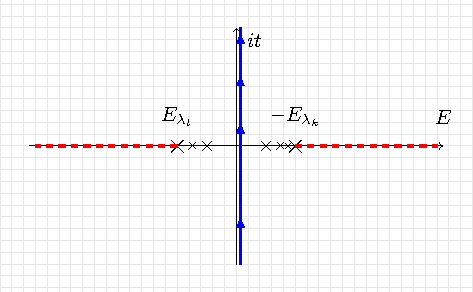
\includegraphics[width=120mm]{Graphs/Contour.pdf} 
			\caption{Diagram of the integration contour used in~\eqref{contour}. Crosses represent poles corresponding to bound states, while red dashed lines represent branch cuts corresponding to the continuous spectrum of free states. There are no poles at $t=0$, as the $\lambda_k$ and $\lambda_l$ states are omitted in the spectral representations of the corresponding reduced Green's functions} \label{degeneracyFig}
		\end{figure}
	
In order to express the double-electron correction however, we need the two-electron reduced hydrogen Green's function with spectral representation of
\begin{equation}
\widetilde{G}_{\lambda_k,\lambda_l}^2 = \sum_{\substack{\sigma_1 \neq \lambda_k\\\sigma_2 \neq \lambda_l}} \frac{|\sigma_1\rangle |\sigma_2\rangle \langle
	\sigma_1| \langle \sigma_2|}{E_{\lambda_k} + E_{\lambda_l} -
	E_{\sigma_1} - E_{\sigma_2}}.\label{eq:16}
\end{equation}
Unfortunately, it does not have a closed form, but borrowing a clever trick from complex analysis we can express it as a convolution over the energy of two single-electron Green's functions
\begin{equation}
\widetilde{G}^{(2)}_{\lambda_k,\lambda_l} (r_1,r_2,r_3,r_4) = \int
\widetilde{G}_{E_{\lambda_k}+it}(r_1,r_2)\widetilde{G}_{E_{\lambda_l}-it}(r_3,r_4)
\frac{dt}{2 \pi i}\label{contour} .
\end{equation}
This somewhat surprising formula follows immediately from applying the
following identity, which is simply a residue theorem for a product of
simple poles, directly to the above spectral representation of the Green's function
\begin{equation}
\int \frac{1}{a+it}\frac{1}{b-it}dt = \frac{-2 \pi}{a+b},\label{eq:18}
\end{equation}
which is valid, provided that both $a$ and $b$ are negative,
which will always be the case in the ground state, as they stand for
differences between the ground state energy and intermediate energies.

With that in mind, the single-electron second order correction can simply be calculated, as
\begin{equation}\label{SecondDouble}
    \Delta E^{(2)}_{\rm{double}} = \sum_{k \neq l} \langle \lambda_k \lambda_l|\widehat{W} \widetilde{G}^{(2)}_{\lambda_k,\lambda_l} \widehat{W}|\lambda_k \lambda_l \rangle,
\end{equation}
where exchange elements are implied according to~\eqref{Exchange}.

\section{Subtractions}

At this point, we still need to take into account the Pauli exclusion principle. It manifests itself in the fact that sums over $\sigma$ in~\eqref{SecondSigma}, do not include occupied single-electron orbitals. This means that despite using reduced Greens functions we still need to subtract all other occupied states.

This means subtracting the following sum from the single-electron second order correction
\begin{equation}
  \sum_{m \neq k \neq l} \frac{|\langle \lambda_k \lambda_l|\widehat{W} |\lambda_k \lambda_m\rangle |^2}{E_{\lambda_l} - E_{\lambda_m}}.
\end{equation}
 And from the double-electron one
\begin{equation}
  \sum_{n \neq m,k \neq l} \frac{|\langle \lambda_k \lambda_l|\widehat{W} |\lambda_m \lambda_n\rangle |^2}{E_{\lambda_l}+E_{\lambda_k} - E_{\lambda_m} - E_{\lambda_n}}.
\end{equation}

However note that all terms in the above sums are anti-symmetric with respect to the $l \rightarrow m$ and $(k,l) \rightarrow (m,n)$ exchanges respectively, so the total amount subtracted from the correction to any multi-electron configuration is equal to zero. This can also serve as a useful check of the consistency of all calculations.

\section{Effects of degeneracy}

Naive application of the above formulas will lead to divergent results for many electronic configurations, even including some of the ground states of neutral atoms. This is because of the high degeneracy of the hydrogen-like basis, in particular the lack of energy dependence on the angular momentum quantum number. It can be readily seen from the formula for the reduced Greens function used in the derivation of the second order energy corrections
\begin{equation}
    G^{\psi_0}=\sum_k\frac{|\psi_k\rangle\langle\psi_k|}{E_{\psi_0}-E_{\psi_k}}.
\end{equation}

This leads to a divergence whenever for any of the virtual states $\psi_k$ we have $E_{\psi_k} = E_{\psi_0}$. It is never the case when calculating single-electron corrections as there are no elements $\langle \psi_k|\widehat{W}|\psi_l\rangle$ with non-zero amplitudes, that change the angular momentum quantum number of exactly one electron. However, it does happen when calculating the double electron correction, for example to the ground state of beryllium, as $\langle 2s 2s|\widehat{W}|2p2p\rangle \neq 0$ (see Figure~\ref{degeneracyFig}).

	\begin{figure}
			\centering
			\includegraphics[width=120mm]{Graphs/degeneracy.png} 
			\caption{Pictorial representation of an example of an intermediate state
				with degenerate energy, causing a divergence in
				the double-electron second order correction to the energy of beryllium. Such transitions do not happen in elements that have at least half-filled outer shells or only a single valance electron e.g. lithium.} \label{degeneracyFig}
		\end{figure}
	
	In order to mitigate this, whenever there are multiple configurations with equal zeroth-order energy, we have to diagonalize the Hamiltonian in the subspace spanned by those configurations and consider it's eigenvectors as the new zeroth-order approximations. On top of regularizing divergences, this further increases the accuracy of the ECM calculation as it effectively includes corrections of all orders coming from those configurations. The resulting zeroth-order wavefunction is then a linear combination of those degenerate configurations. For example the ground state configuration of berylium becomes\footnote{We show approximate coefficients for clarity, but they can be calculated as exact analytical numbers within the ECM.} $0.9743|1s^22s^2\rangle + 0.2252|1s^22p^2\rangle$.
	
	This means that we have more contributions to the second-order correction in such cases, as now transitions to all virtual states that differ by no more than two electrons from any of the zeroth order degenerate basis states have to be taken into account.  It is important to note, that all of those configurations differ by exactly two electrons (for reasons mentioned above). So for a wavenuction
	\begin{equation}
    |\psi\rangle = \sum_i \alpha_i |\lambda^i_1...\lambda^i_n \rangle = \sum_i \alpha_i |\lambda_1...\lambda_{n-2} \chi_1^i \chi_2^i \rangle,
\end{equation}
we get the correction
\begin{align}
    \Delta E^{(2)}_{\rm{single}} =& \sum_{m \neq l \neq k}^{n} \sum_i\alpha_i^2 \langle \lambda^i_k \lambda^i_l|\widehat{W} |\lambda^i_k \widetilde{G}_{\lambda^i_l} \lambda^i_m|\widehat{W}|\lambda^i_l \lambda^i_m \rangle \nonumber 
    \\
    &+\sum_{i,j}\sum_{k} \alpha_i \alpha_j\langle \lambda_k \chi^i_1|\widehat{W} |\lambda_k \widetilde{G}_{\lambda} \chi^i_2|\widehat{W}|\chi^j_1 \chi^j_2 \rangle \nonumber
    \\
    & + \sum_{i,j}\sum_{k} \alpha_i \alpha_j\langle \lambda_k \chi^i_1|\widehat{W} |\chi^j_1 \widetilde{G}_{\lambda} \chi^i_2|\widehat{W}|\chi^j_2 \lambda_k \rangle \nonumber 
    \\
    &+ \sum_{i,j}\sum_{k \neq l} \alpha_i \alpha_j \frac{\langle \lambda_k \lambda_l|\widehat{W} |\chi^i_1\chi^i_2 \rangle\langle \lambda_k \lambda_l |\widehat{W}|\chi^j_1 \chi^j_2 \rangle}{E_k+E_l-2E_{\chi}}.
\end{align}
Similarly, the double electron correction becomes
\begin{align}
    \Delta E^{(2)}_{\rm{double}} =& \sum_i \sum_{k \neq l} \alpha_i^2 \langle \lambda^i_k \lambda^i_l|\widehat{W} \widetilde{G}^{(2)}_{\lambda^i_k,\lambda^i_l} \widehat{W}|\lambda^i_k \lambda^i_l \rangle \nonumber \\
    &+ \sum_{i \neq j}  \alpha_i \alpha_j \langle \chi^i_1 \chi^i_2|\widehat{W} \widetilde{G}^{(2)}_{\chi^i_1,\chi^i_2} \widehat{W}|\chi^j_1 \chi_j^2 \rangle,
\end{align}
where the subtractions in all Greens functions now include all states contained in any of the degenerate configurations.


\section{Closed subshells}

Finally we want to show closed form formulas for the summation over projections of angular momenta. Using the generalized orthogonality relation of 3-$j$ symbols~\cite{cowan1981theory}
\begin{align} \label{3jProps2}
    \sum_m (-1)^m\begin{pmatrix} l & l & k \\ -m & m & 0\end{pmatrix} = (-1)^l\delta_{k,0}\sqrt{2l+1}&, \\
    \sum_{m_1,m_2}
    \begin{pmatrix} l & l_1 & l_2 \\ m_1-m_2 & -m_1 & m_2 \end{pmatrix}
    \begin{pmatrix} k & l_1 & l_2 \\ m_2-m_1 & m_1 & -m_2 \end{pmatrix}
    &= \frac{\delta_{l,k}}{2l+1},
\end{align}
we can immediately obtain the formula for the direct term of the single-electron second-order correction:
\begin{align}
    \sum_{m_k,m_l,m_m}\langle \lambda_k |\langle\lambda_l|\widehat{W} |\lambda_k \widetilde{G}_{\lambda_l} &\lambda_m|\widehat{W}|\lambda_l \rangle |\lambda_m \rangle \nonumber \\
    &= (2l_k+1)(2l_m+1)(2l_l+1)I^{\lambda_k,\lambda_l,\lambda_k,\lambda_m,\lambda_l,\lambda_m}_{l_l,0,0},
\end{align}
and the two distinct exchange terms:
\begin{align}
    \sum_{m_k,m_l,m_m}&\langle \lambda_l |\langle\lambda_k|\widehat{W} |\lambda_k \widetilde{G}_{\lambda_l} \lambda_m|\widehat{W}|\lambda_l \rangle |\lambda_m \rangle \nonumber
    \\
    &=\sum_p(2l_k+1)(2l_m+1)(2l_l+1)
    \times\begin{pmatrix} l_k & l_l & p \\ 0 & 0 & 0 \end{pmatrix}^2I^{\lambda_l,\lambda_k,\lambda_k,\lambda_m,\lambda_l,\lambda_m}_{l_l,p,0},
\end{align}
\begin{align}
    \sum_{m_k,m_l,m_m}&\langle \lambda_l |\langle\lambda_k|\widehat{W} |\lambda_k \widetilde{G}_{\lambda_l} \lambda_m|\widehat{W}|\lambda_m \rangle |\lambda_l \rangle \nonumber 
    \\
    &= \sum_{p_1,p_2}(2l_k+1)(2l_m+1)\begin{pmatrix} l_k & l_l & p_1 \\ 0 & 0 & 0 \end{pmatrix}^2\begin{pmatrix} l_m & l_l & p_2 \\ 0 & 0 & 0 \end{pmatrix}^2I^{\lambda_l,\lambda_k,\lambda_k,\lambda_m,\lambda_l,\lambda_m}_{l_l,p_1,p_2},
\end{align}
where the radial integrals are of the form
\begin{align}
    I^{\lambda1,\lambda2,\lambda3,\lambda4,\lambda5,\lambda6}_{p,k,k'} = \int R_{\lambda2}(r)R_{\lambda5}(r')W^k_{\lambda1,\lambda3}(r)W^{k'}_{\lambda4,\lambda6}(r') G_{\lambda_2,p}(r,r')dr dr',
\end{align}
with the potential generated by the electron-electron repulsion defined as
\begin{equation}
    W^k_{\lambda1,\lambda2}(r) = \int R_{\lambda1}(r')R_{\lambda2}(r') \frac{\min[r,r']^k}{\max[r,r']^{k+1}}dr'.
\end{equation}

The analogous calculation for the double-electron contribution is only slightly more involved. Lets first consider an exchange energy between two subshells. For closed subshells $\lambda \neq \lambda'$
\begin{equation}
    \Delta E^{(2)}_{\rm{double}} = \sum_{m,m'}(\langle \lambda \langle \lambda'|\widehat{W} GG \widehat{W}|\lambda \rangle \lambda'\rangle-\delta_{s,s'}\langle \lambda \langle \lambda'|\widehat{W} GG \widehat{W}|\lambda' \rangle \lambda \rangle),
\end{equation}
where the Kronecker delta is 1 if the spins are aligned and 0 otherwise, and we have explicitly expanded the exchange symmetry.

For the case of $\lambda=\lambda'$ we have
\begin{align}
    \Delta E^{(2)}_{\rm{double}} &= \sum_{m>m'}(\langle \lambda_m \lambda_{m'}|\widehat{W} GG \widehat{W}|\lambda_m \lambda_{m'}\rangle-\langle \lambda_{m} \lambda_{m'}|\widehat{W} GG \widehat{W}|\lambda_{m'} \lambda_{m} \rangle) \nonumber\\
    &= \frac{1}{2} \sum_{m,m'}(\langle \lambda_m \lambda_{m'}|\widehat{W} GG \widehat{W}|\lambda_m \lambda_{m'}\rangle-\langle \lambda_{m} \lambda_{m'}|\widehat{W} GG \widehat{W}|\lambda_{m'} \lambda_{m} \rangle).
\end{align}
where we have used the $m \leftrightarrow m'$ symmetry and the fact that the case $m=m'$ cancels out. Therefore we can see that the only difference between those cases is the factor of $1/2$, wchich is related to the exchange antisymmetry of single-electron states.

Using~\eqref{3jProps2} we get the sum over projections in the direct term as
\begin{align}
    &\sum_{m,m'}\langle \lambda \lambda'|\widehat{W} GG \widehat{W}|\lambda \lambda'\rangle \nonumber \\
    &= \sum_{p,q,k} \frac{(2l+1)(2l'+1)(2p+1)(2q+1)}{(2k+1)^2}\left(\begin{matrix}l&p&k\\0&0&0\end{matrix}\right)^2\left(\begin{matrix}l'&q&k\\0&0&0\end{matrix}\right)^2I^{\lambda,\lambda',\lambda,\lambda'}_{p,q,k,k},
\end{align}
where the radial integrals are of the form
\begin{align}
    I^{\lambda1,\lambda2,\lambda3,\lambda4}_{p,q,k,k'} =& \int R_{\lambda1}(r_1)R_{\lambda2}(r_2)R_{\lambda3}(r_3)R_{\lambda4}(r_4) G^{\lambda}_{p,t}(r_1,r_3)G^{\lambda'}_{q,-t}(r_2,r_4) \nonumber\\
    &\times \frac{\min[r_1,r_2]^k}{\max[r_1,r_2]^{k+1}}\frac{\min[r_3,r_4]^{k'}}{\max[r_3,r_4]^{k'+1}}dr_1dr_2dr_3dr_4dt.
\end{align}

 Similarly, we can sum over projections in the calculation of the exchange element, using the definition of the 6-$j$ symbol~\cite{cowan1981theory}
\begin{align}
   \sum_{m_1...m_6}(-1)^\xi&\left(\begin{matrix}j_1&j_2&j_3\\-m_1&-m_2&-m_3\end{matrix}\right)\left(\begin{matrix}j_1&j_5&j_6\\m_1&-m_5&m_6\end{matrix}\right) \nonumber\\
   &\times\left(\begin{matrix}j_4&j_2&j_6\\m_4&m_2&-m_6\end{matrix}\right)\left(\begin{matrix}j_4&j_5&j_3\\-m_4&m_5&m_3\end{matrix}\right) =  \bigg\{\begin{matrix}j_1&j_2&j_3\\j_4&j_5&j_6\end{matrix}\bigg\},
\end{align}
where $\xi = \sum_i (j_i-m_i)$. The final expression comes out as
\begin{align}
    \sum_{m,m'}\langle \lambda \lambda'|\widehat{W} GG \widehat{W}|\lambda' \lambda\rangle =& \sum_{p,q,k,k'} (2l+1)(2l'+1)(2p+1)(2q+1) \nonumber\\
    &\times\left(\begin{matrix}l&p&k\\0&0&0\end{matrix}\right)\left(\begin{matrix}l&q&k'\\0&0&0\end{matrix}\right)\left(\begin{matrix}l'&p&k'\\0&0&0\end{matrix}\right) \nonumber
    \\
    &\times\left(\begin{matrix}l'&q&k\\0&0&0\end{matrix}\right)\bigg\{\begin{matrix}l&p&k\\l'&q&k'\end{matrix}\bigg\}I^{\lambda,\lambda',\lambda',\lambda}_{p,q,k,k'}.
\end{align}

Since the resulting formulas are somewhat involved, it is instructive to look at the first few examples. For the case of $\lambda\neq\lambda'$ we get the correlations between the $s$ and $p$ shells:
\begin{align}
    \lambda_s,\lambda'_s &: \Delta E^{(2)}_{\rm{double}}= \sum_a \frac{2a+1}{16 \pi^2} (I^{\lambda,\lambda',\lambda,\lambda'}_{a,a,a,a} - I^{\lambda,\lambda',\lambda',\lambda}_{a,a,a,a}) \\
    \lambda_s,\lambda'_p &:\Delta E^{(2)}_{\rm{double}}= \sum_a \frac{3(a+1)}{16 \pi^2} (I^{\lambda,\lambda',\lambda,\lambda'}_{a,a+1,a,a}+I^{\lambda,\lambda',\lambda,\lambda'}_{a+1,a,a,a} \\
    &+ I^{\lambda,\lambda',\lambda,\lambda'}_{a+1,a,a+1,a+1}+I^{\lambda,\lambda',\lambda,\lambda'}_{a,a+1,a+1,a+1}-I^{\lambda,\lambda',\lambda',\lambda}_{a+1,a,a+1,a}-I^{\lambda,\lambda',\lambda',\lambda}_{a,a+1,a,a+1}) \\
  \lambda_p,\lambda'_p &:\Delta E^{(2)}_{\rm{double}}= \frac{9}{16\pi^2}\sum_a [\frac{(a+1)^2}{(2a+1)}I^{\lambda,\lambda',\lambda,\lambda'}_{a+1,a+1,a,a} +\frac{(a+1)^2}{(2a+3)}I^{\lambda,\lambda',\lambda,\lambda'}_{a,a,a+1,a+1} \\
  &-\frac{a+1}{(2a+1)(2a+3)}(I^{\lambda,\lambda',\lambda',\lambda}_{a+1,a+1,a,a} +I^{\lambda,\lambda',\lambda',\lambda}_{a,a,a+1,a+1}) \\
 &+2 \frac{(a+1)(a+2)}{(2a+3)}(I^{\lambda,\lambda',\lambda,\lambda'}_{a,a+2,a+1,a+1}-I^{\lambda,\lambda',\lambda',\lambda}_{a+1,a+1,a,a+2} -I^{\lambda,\lambda',\lambda',\lambda}_{a,a+2,a+1,a+1})]
\end{align}
where the exchange parts should be skipped if $\lambda$ and $\lambda'$ have opposite spins.

On the other hand when $\lambda=\lambda'$ the same terms read:
\begin{align}
    \lambda_s,\lambda_s &: \Delta E^{(2)}_{\rm{double}}= 0 \\
  \lambda_p,\lambda_p &: \Delta E^{(2)}_{\rm{double}}= \frac{9}{32\pi^2}\sum_a (a+1)[\frac{a}{2a+1}I^{\lambda,\lambda',\lambda,\lambda'}_{a,a,a+1,a+1}\nonumber
  \\
  &+\frac{(a+2)}{(2a+3)}(I^{\lambda,\lambda',\lambda,\lambda'}_{a+1,a+1,a,a}-2I^{\lambda,\lambda',\lambda',\lambda}_{a+1,a+1,a,a+2})]
\end{align}


Since these are independent of charge in the Schr\"odinger theory, the values of $I$ integrals can easily be tabulated for all possible parameters. %Tabulate?